\documentclass[11pt]{article}
\usepackage{natbib}
\usepackage{graphicx}
\usepackage{subcaption}
\usepackage{amsmath}
\usepackage{amsfonts}
\usepackage{enumitem}
\usepackage{setspace}
\usepackage{booktabs}
\usepackage{tabulary}
\usepackage{hyperref}
\usepackage[capitalise,noabbrev]{cleveref}
\usepackage[a4paper, total={6in, 8in}]{geometry}
\usepackage{tikz}
\usetikzlibrary{shapes,arrows,positioning}

\tikzset{
    %Define standard arrow tip
    >=stealth',
    %Define style for boxes
    block/.style={
           rectangle,
           draw=black,
           text width=6.5em,
           minimum height=3em,
           text centered},
    % Define arrow style
    arrow/.style={
           ->,
           thick,
           shorten <=2pt,
           shorten >=2pt,
           }
}

\bibliographystyle{plainnat}
\setcitestyle{authoryear,open={(},close={)}}

\newcommand{\pkg}[1]{{\fontseries{b}\selectfont #1}} 


\title{\textbf{A path model of energy intensity}}
\author{S. Drake Siard}
\date{2020 May 5}
\begin{document}

\maketitle

\begin{abstract}
This project aims to further develop a published path model, originally applied to Bangladesh, to analyse the direct and indirect impacts of growth, industrialization, technological innovation, and trade openness on energy intensity.
The model is first validated by replicating the results in the original paper, and some choices regarding model construction and data treatment are re-assessed.
A modified version of the model then applied to more recent data in India and the UK, where the directions of industrialisation and technological innovation differ, to see if the original hypotheses hold.

Word count: \em{Drake forgot to do this!}
 
\end{abstract}

\tableofcontents

\pagebreak

\section{Introduction}\label{sec:introduction}

Energy intensity, defined as the demand for energy per unit of output, is a critical measure of economic efficiency; it becomes every more important as the world economy develops and world populations continue to rise.
Decreasing energy intensity is a necessary condition for the developing world's economic growth to continue through this century without overwhelming the world's limited resources, and for the developed world to maintain its quality of life while reducing their energy consumption.

\cite{panHowIndustrializationTrade2019} cite an extensive literature on energy intensity and its influencing factors, and extract four commonly described determinants of energy intensity: industrialization, trade openness, technological innovation, and economic growth.
These nature of these variables, and the specific economic data series used to represent them, are described in greater detail in \cref{sec:data_sources}.
They note that due to the interdependence of these variables there may both direct and indirect effects, and propose a path model (which they describe as novel) to analyse these effects; this model is described and the results analysed in \cref{sec:original_model}.
The model is used to test four hypotheses:
\begin{enumerate}[label=\textbf{H.\arabic*}]
\item Industrialisation has positive direct impact on energy intensity.
\item Industrialization has negative indirect impact on energy intensity through technological innovation.
\item Trade openness has negative direct impact on energy intensity.
\item Trade openness has negative indirect impact on energy intensity through economic growth.
\end{enumerate}


\section{Data Sources}\label{sec:data_sources}
 
As in \cite{panHowIndustrializationTrade2019}, the dependent variable is energy intensity (denoted EI). The two independent variables are level of industrialization (ISG)\footnote{
The abbreviation is due to the original paper labelling this as ``Industrial Share of Growth"; however, the measure actually used is industrial share of output, not of output growth. 
Similarly, the variable P\_GDP is a measure of output per capita, not growth.
} and trade openness (TO), and the two intermediary variables are economic output (P\_GDP) and technological innovation (TI).
The precise definitions\footnote{
Supplementing Table 2 in \cite{panHowIndustrializationTrade2019}
} are described in \cref{tab:data_source}.
All data is sampled at an annual frequency.
The specific energy intensity measure in this case is not directly available form the database in those units, but is constructed by taking the primary energy use in kg. of oil equivalent per capita, divided by the (2015, PPP-adjusted) \$US GDP per capita.

\begin{table}[htbp]
\centering
\begin{tabulary}{\textwidth}{l l L} 
 \toprule 
 Abbr. & Name & Description and units \\ [1ex] 
 \midrule 
 EI & Energy intensity & Primary energy use in kg. of oil equivalent per ``current" (2018 or 2019, by vintage) \$US of GDP \\ 
 EIb & Energy intensity (alt.) & Primary energy use in kg. of oil equivalent per (2015, PPP-adjusted) \$US of GDP \\ 
 ISG & Industrialisation & Total industry (mining, construction, utilities) value added as \% of GDP \\
 TO & Trade openness & Total value of imports and exports (goods and services) as \% of GDP \\ 
 TI & Technological innovation & Total number of patent applications (direct and PCT national phase entries) \\ 
 P\_GDP & Economic output & GDP in ``current" (2018 or 2019, by dataset) \$US, divided by mid-year population \\ 
 \bottomrule 
\end{tabulary}
\caption{Variable names and descriptions}
\label{tab:data_source}
\end{table}

For the replication phase, in order to most closely match \cite{panHowIndustrializationTrade2019}, it was necessary\footnote{
ISG was revised in the June 2018 vintage, and the ``current" \$US scaler for P\_GDP was rebased in September 2019.
} to use the April 2018 vintage of the data from the WDI Database Archives, \cite{theworldbankWDIDatabaseArchives2018}.
Additional patent data was retrieved directly from the WIPO Statistics Database via the IP Statistics Data Center, \cite{wipoWIPOStatisticsDatabase2020}, and used to fill in gaps in World Bank data where necessary.

For the updated analysis, data was taken directly from the most recent update of the WDI database, \cite{theworldbankWorldDevelopmentIndicators2019}. In addition, an up-to-date alternate energy intensity measure was added from \cite{enerdataGlobalEnergyStatistical2019} and denoted EIb in the dataset.

In the original paper, the data truncated to the date range 1986-2015, but subject to no further transformation, resulting in the summary statistics in \cref{tab:original_summary_stats} and variable correlations in \cref{fig:original_summary_corr};
significant correlations (at the 0.01 level) are denoted with an asterisk.
Comparing these with the Table 3 and Table 4 of \cite{panHowIndustrializationTrade2019}, there is a close match but not an exact one.
Of some concern is the mismatch in the number of samples of EI: the per capita primary energy use measure used to construct it is absent for the year 2015, in both previous vintages and the current version of the upstream database.
While we can incomplete data to estimate the model, this will result in an additional difference with the original paper.

\begin{table}[htbp]
\centering
\begin{tabular}{lrrrrr}
\toprule
{} &    min &     max &   mean &    std &  count \\
\midrule
ISG   &  20.05 &   28.15 &  24.07 &   2.28 &     30 \\
TO    &  16.69 &   48.11 &  30.56 &   9.98 &     30 \\
TI    &  93.00 &  354.00 & 239.20 &  93.50 &     30 \\
P\_GDP & 227.42 & 1210.16 & 498.83 & 261.51 &     30 \\
EI    &   0.20 &    0.49 &   0.35 &   0.07 &     29 \\
\bottomrule
\end{tabular}
\caption{Original data summary statistics}
\label{tab:original_summary_stats}
\end{table}


\begin{figure}[htbp]
\centering
\includegraphics[width=\textwidth]{./plots/BGD_201805_correlations.pdf}
\caption{Original data correlations}
\label{fig:original_summary_corr}
\end{figure}

\section{Original Model}\label{sec:original_model}

Path models\footnote{ 
This is a summary of material in \cite{klinePrinciplesPracticeStructural2016}; the interested reader is directed to the source for more details.
} are a subset of structural equation models that deal only with observed variables (as opposed to hidden, or latent variables), where between the exogenous and final endogenous variables there may be one or more mediating endogenous variables.
In the case of this model, openness to trade and industrialisation are the exogenous variables; openness to trade  

This model is represented\footnote{
Following Figure 3 in \cite{panHowIndustrializationTrade2019}, we simplify the diagram by dropping the variance notation.
} in \cref{fig:original_model}. 

Variance of the exogenous 

The sample size ($n=30$) is at the very lower bound of what might be considered acceptable for SEM.

\begin{figure}[htbp]
\centering
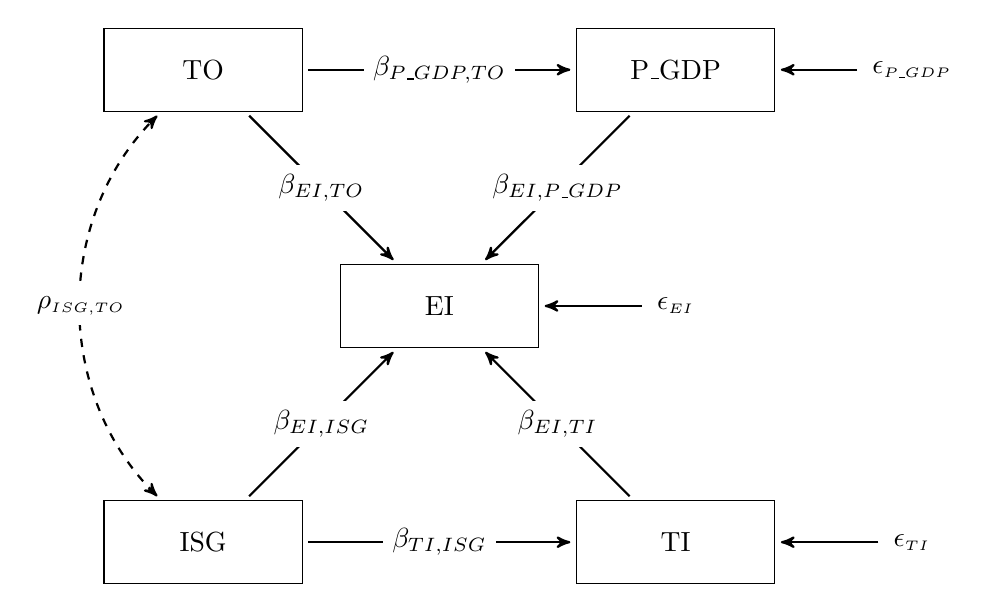
\begin{tikzpicture}[node distance = 3cm, auto]
    \node [block] (EI) {EI};
    \node [above of=EI] (upper dummy) {};    
    \node [below of=EI] (lower dummy) {};    
    \node [block, left of=upper dummy] (TO) {TO};
    \node [block, left of=lower dummy] (ISG) {ISG};
    \node [block, right of=upper dummy] (PGDP) {P\_GDP};
    \node [block, right of=lower dummy] (TI) {TI};
    \node [right of=PGDP] (epsPGDP) {$\epsilon_{\scriptscriptstyle{P\_GDP}}$};
    \node [right of=EI] (epsEI) {$\epsilon_{\scriptscriptstyle{EI}}$};
    \node [right of=TI] (epsTI) {$\epsilon_{\scriptscriptstyle{TI}}$};

	\path[->] (ISG) edge[arrow] node[anchor=center, fill=white] {$\beta_{EI,ISG}$} (EI);
	\path[->] (ISG) edge[arrow] node[anchor=center, fill=white] {$\beta_{TI,ISG}$} (TI);
	\path[->] (TO) edge[arrow] node[anchor=center, fill=white] {$\beta_{EI,TO}$} (EI);
	\path[->] (TO) edge[arrow] node[anchor=center, fill=white] {$\beta_{P\_GDP,TO}$} (PGDP);
	\path[->] (PGDP) edge[arrow] node[anchor=center, fill=white] {$\beta_{EI,P\_GDP}$} (EI);
	\path[->] (TI) edge[arrow] node[anchor=center, fill=white] {$\beta_{EI,TI}$} (EI);
	\path[->] (epsPGDP) edge[arrow] (PGDP);
	\path[->] (epsEI) edge[arrow] (EI);	
	\path[->] (epsTI) edge[arrow] (TI);
	\path (ISG) 
		edge[arrow, <->, bend left=45, dashed] 
		node[anchor=center, fill=white] {$\rho_{\scriptscriptstyle{ISG,TO}}$} 
		(TO);
\end{tikzpicture}
\caption{Path model for EI, mediated by P\_GDP and TI}
\label{fig:original_model}
\end{figure}






This model was fitted using an R software package for latent variable modeling called \pkg{lavaan}, \cite{rosseelLavaanPackageStructural2012}, and supplementary analysis was performed using the \pkg{semTools} package, \cite{jorgensenSemToolsUsefulTools2019}.\footnote{
Additional code for generating model predictions and residuals was drawn from user contributions that have not yet been merged with the main \pkg{semTools} codebase.
See \url{https://github.com/simsem/semTools/pull/25} and \url{https://github.com/simsem/semTools/compare/master...drakesiard:residual-predict} for more detail.
}

Fit measures described in \cite{parryFitIndicesCommonly2020}.

\section{Data Analysis}

\section{Revised Model}

\section{Conclusion}
Maybe.

\clearpage

\appendix

\renewcommand{\refname}{\section{References}}.
\bibliography{project}


\section{Appendices}


\subsection{Another appendix}

More lipsum.

\end{document}



\end{document}
